\documentclass[12pt,a4paper]{article}
\usepackage[a4paper,top=1.5cm, bottom=1.5cm, left=1.5cm, right=1.5cm]{geometry}
\usepackage[T2A]{fontenc}
\usepackage[utf8]{inputenc}
\usepackage[russian]{babel}
\usepackage{amsmath}
\usepackage{amssymb}
\usepackage{graphicx}
\usepackage{floatrow}
\usepackage{booktabs}
\usepackage{wrapfig}
\usepackage{indentfirst}
\usepackage{lipsum}
\usepackage{subcaption}
\usepackage{float}
\usepackage{enumitem}
\restylefloat{table}

\newcommand{\figref}[1]{(см. рис. \ref{#1})}
\newcommand{\e}[1]{\text{$\cdot10^{#1}$}}

\title{Лабораторная работа 5.2.3 \\ Изучение спектра поглощения молекулярного йода}
\author{Симанкович Александр\\ Б01-108}
\date{28.10.2023}

\begin{document}
	\maketitle
	
	\section*{Аннотация}
	
	В работе проведено экспериментальное измерение спектра поглощения молекулярного йода. Получены серии Деландра. Измерено значение кванта колебательных возбуждений молекулы йода в возбужденном состоянии $h \nu_2 = (12.0 \pm 0.7) \text{ мэВ}.$ Оценено значение кванта колебательных возбуждений $ h \nu_1 = (10 \div 100) \text{ мэВ}$. Также вычислено значение энергии электронного перехода $E_2 - E_1 = (2.17 \pm 0.02) \text{ эВ}.$
	
%	В работе экспериментально подтвержден эффект электронного парамагнитного резонанса в молекуле дифенилпикрилгидразила (ДФПГ). Подтверждена теоретическая зависимость резонансной частоты от значения магнитного поля. Получен $g$-фактор несвязанного электрона в молекуле ДФПГ $g = (1.94 \pm 0.04)$ . Оценено время релаксации электрона в молекуле ДФПГ $\tau = (15.0 \pm 1.0)$ нс.
	
	\section*{Теоретическое введение}
	
	\subsection*{Спектр возбужденных состояний молекулы}
	
	Изолированные атомы обладают дискретным спектром, который формируется из переходов электронов на более высокие энергетические уровни. В молекулах, в отличие от атомов, могут возбуждаться дополнительные степени свободы: колебательные и вращательные. В первом приближении, не учитывая взаимное влияние возбуждения электронов и дополнительных степеней свободы, получаем:
	$$ E = E_{\text{эл}} + E_{\text{колеб}} + E_{\text{вращат}}$$
	$$ \psi = \psi_{\text{эл}} \cdot \psi_{\text{колеб}} \cdot \psi_{\text{вращат}} $$
	
	Таким образом, энергию молекулы можно рассматривать как отдельные компоненты, связанные с возбуждением электронов, колебаниями атомов в молекуле и вращением молекулы вокруг своих осей.

	\subsection*{Масштабы составляющих энергии}
	
	\subsubsection*{Электронные термы}
	
	Энергетические уровни молекул, -- \textit{термы}, связанные с переходами электронов, по происхождению идентичны электронным термам атомов. Но из-за взаимодействия с другими атомами, формирующими так называемое \textit{внутреннее электрическое поле}, эти уровни расщепляются. Аналогичный эффект возникает при помещении атома во внешнее электрическое поле (эффект Штарка).
	
	Характерная энергия электронных термов:
	\begin{equation}
		\hbar \omega_{\text{эл}} \approx R_y \sim 10 \text{ эВ}
	\end{equation}
	
	\subsubsection*{Энергия колебаний}
	
	Потенциал взаимодействия двух атомов представляет собой потенциальную яму с минимумом в точке $r_0$.
	
	\begin{figure}[H]
		\centering
		\includegraphics[width=0.6\linewidth]{res/ocsillation_levels.png}
		\caption{Схема энергетических уровней двухатомной молекулы.}
		\label{fig:oscillation_levels}
	\end{figure}
	
	В молекуле могут возникать колебания атомов. Поскольку вблизи минимума потенциальная яма описывается параболой, нижние уровни энергии можно считать уровнями энергии гармонического осциллятора:
	\begin{equation}
		E_{\text{колеб}} = \hbar \omega_0 (n + \frac{1}{2})
	\end{equation}
	
	Как можно видеть, уровни энергии являются равноотстоящими. При увеличении энергии начинает влиять \textit{ангармонизм} -- отступление от гармонического закона. Это приводит к изменению разностей энергии между уровнями.
	
	Оценим энергию колебаний. Будем считать, что при смещении на расстояние порядка боровского радиуса $a_0$ изменение потенциальной энергии составляет порядка $R_y$. Тогда получим:
	\begin{equation}
		U \sim \frac{(r - r_0)^2}{a_0^2} R_y + U(r_0) \quad \Rightarrow \quad k \sim \frac{R_y}{a_0^2}
	\end{equation}
	Для частоты колебаний:
	\begin{equation}
		\omega_{\text{колеб}} = \sqrt{\frac{k}{M}} \sim \alpha^2 \frac{mc^2}{\hbar} \sqrt{\frac{m}{M}}
	\end{equation}
	
	Сравним с электронными термами:
	\begin{equation}
		\omega_{\text{эл}} \sim \frac{R_y}{\hbar} \approx \alpha^2 \frac{mc^2}{\hbar} \quad \Rightarrow \quad \frac{E_{\text{колеб}}}{E_{\text{эл}}} \sim 10^{-3}
	\end{equation}
	
	Таким образом, формируется расщепление электронных терм.
	
	\subsubsection*{Энергия вращения}
	
	Каждая молекула имеет дискретный набор состояний, соответствующий вращению вокруг некоторой оси как целого. Оценим энергию этой степени свободы.
	$$ J = ma_0^2, $$
	где $J$ -- момент инерции относительно центра масс молекулы для оси, перпендикулярной оси молекулы.
	Энергия вращения квантуется:
	$$ E_{\text{вращ}} = \frac{\hbar^2}{2J} l(l+1) $$
	
	Сравнивая с электронными термами:
	\begin{equation}
		E_{\text{вращ}} \approx \frac{\hbar^2}{J} \approx \frac{\hbar^2}{Ma_0^2} \quad \Rightarrow \quad \frac{E_{\text{вращ}}}{E_{\text{эл}}} \approx \frac{m}{M},
	\end{equation}
	где $m$ -- масса электрона, $M$ -- масса молекулы.
	Итоговая оценка:
	\begin{equation}
		\omega_{\text{эл}} : \omega_{\text{колеб}} : \omega_{\text{вращ}} \sim 1 : \sqrt{\frac{m}{M}} : \frac{m}{M} \sim 1 : 10^{-3} : 10^{-6}
		\label{eq:relation}
	\end{equation}
	
	\subsection*{Наблюдаемые спектры}
	
	Оптические спектрометры работают в диапазонах энергий, соответствующим электронным термам ($E \sim 1$ эВ). Исходя из оценки \eqref{eq:relation} видно, что оптические спектрометры ($R \sim 1000$) не в состоянии наблюдать вращательные переходы. Таким образом, в полученных спектрах будут наблюдаться переходы между электронными уровнями, на которые наложены спектры колебательных степеней свободы \figref{fig:term_pair}.
	
	\begin{figure}[H]
		\centering
		\includegraphics[width=0.6\linewidth]{res/term_pair.png}
		\caption{Электронно-колебательные уровни двухатомной молекулы.}
		\label{fig:term_pair}
	\end{figure}
	
	Штриховкой обозначен сплошной спектр, возникший из-за ангармонизма потенциала. На рисунке также обозначены некоторые характерные энергии:
	$D_1, D_2$ -- энергии диссоциации для двух электронных терм, $h\nu_{\text{эл}}$ -- энергия электронного перехода, $E_a$ -- энергия возбуждения атома (переход из непрерывного спектра электронного терма 1 в непрерывный спектр электронного терма 2).
	
	Рассмотрим переходы молекулы йода $I_2$ в оптическом диапазоне. Все возможные переходы между колебательными уровнями соседних электронных состояний можно разбить на \textit{серии Деландра} \figref{fig:delandr_series}.
	\begin{figure}[H]
		\centering
		\includegraphics[width=0.6\linewidth]{res/delandr_series.png}
		\caption{Электронно-колебательный спектр молекулы йода.}
		\label{fig:delandr_series}
	\end{figure}
	Интенсивность каждой серии пропорциональна количеству частиц на колебательном уровне основного электронного состояния. В соответствии с распределением Больцмана получаем:
	$$ N \sim e^{\frac{E}{kT}} \quad \Rightarrow \quad N_0 : N_1 : N_2 \approx 1 : \frac{1}{3} : \frac{1}{10}. $$
	
	Энергетические положения линий:
	\begin{equation}
		h \nu_{0, n_2} = (E_2 - E_1) + h \nu_2 (n_2 + \frac{1}{2}) - \frac{1}{2} h \nu_1
		\label{eq:lines}
	\end{equation}
	
	Очевидно, что расстояния между линиями будут равны $h \nu_2$. Следующая серия сдвинута в направлении меньших энергий на $h \nu_1$.
	
	В итоге мы получаем наложение нулевой и первой серий Деландра.
	
	\begin{figure}[H]
		\centering
		\includegraphics[width=0.6\linewidth]{res/spectrum.png}
		\caption{Спектр поглощения паров йода.}
		\label{fig:spectrum}
	\end{figure}
	
	\section*{Методика эксперимента}
	
	\begin{figure}[H]
		\centering
		\begin{minipage}{0.4\textwidth}
			\centering
			\includegraphics[width=0.9\linewidth]{res/setup.png}
		\end{minipage}%
		\begin{minipage}{0.6\textwidth}
			\centering
			\includegraphics[width=0.9\linewidth]{photos/setup.png}
		\end{minipage}
		\caption{Схема установки для изучения спектра поглощения паров йода.}
		\label{fig:coil}
	\end{figure}
	
	Изучение спектра производится с помощью монохроматора и фотокамеры, закрепленной в его окуляре. Изображение с камеры выводится на экран компьютера, где производится дальнейшая обработка.
	
	Сначала производится калибровка монохроматора с помощью неоновой лампы. После этого на стойку устанавливается кювета с йодом и лампа накаливания. Йод в лампе разогревается с помощью электронагревателя до парообразного состояния. 
	
	\section*{Результаты}
	
	\subsection*{Калибровка монохроматора}
	
	На стойку ставится неоновая лампа, ее четкое изображение формируется на входной щели монохроматора с помощью конденсора. Поскольку калибровка производится для обработки данных с фотографий, лимб монохроматора и линза объектива монохроматора после настройки зафиксированы на все время эксперимента. 
	
	Чувствительность камеры (ISO) выставлена в минимальное значение для уменьшения шумов. Производится пара снимков: с длинной ($1$ с) и короткой выдержкой ($1/50$ с).
	
	\begin{figure}[H]
		\centering
		\begin{minipage}{0.5\textwidth}
			\centering
			\includegraphics[width=0.9\linewidth]{data/323_1s/323_1s.jpg}
		\end{minipage}%
		\begin{minipage}{0.5\textwidth}
			\centering
			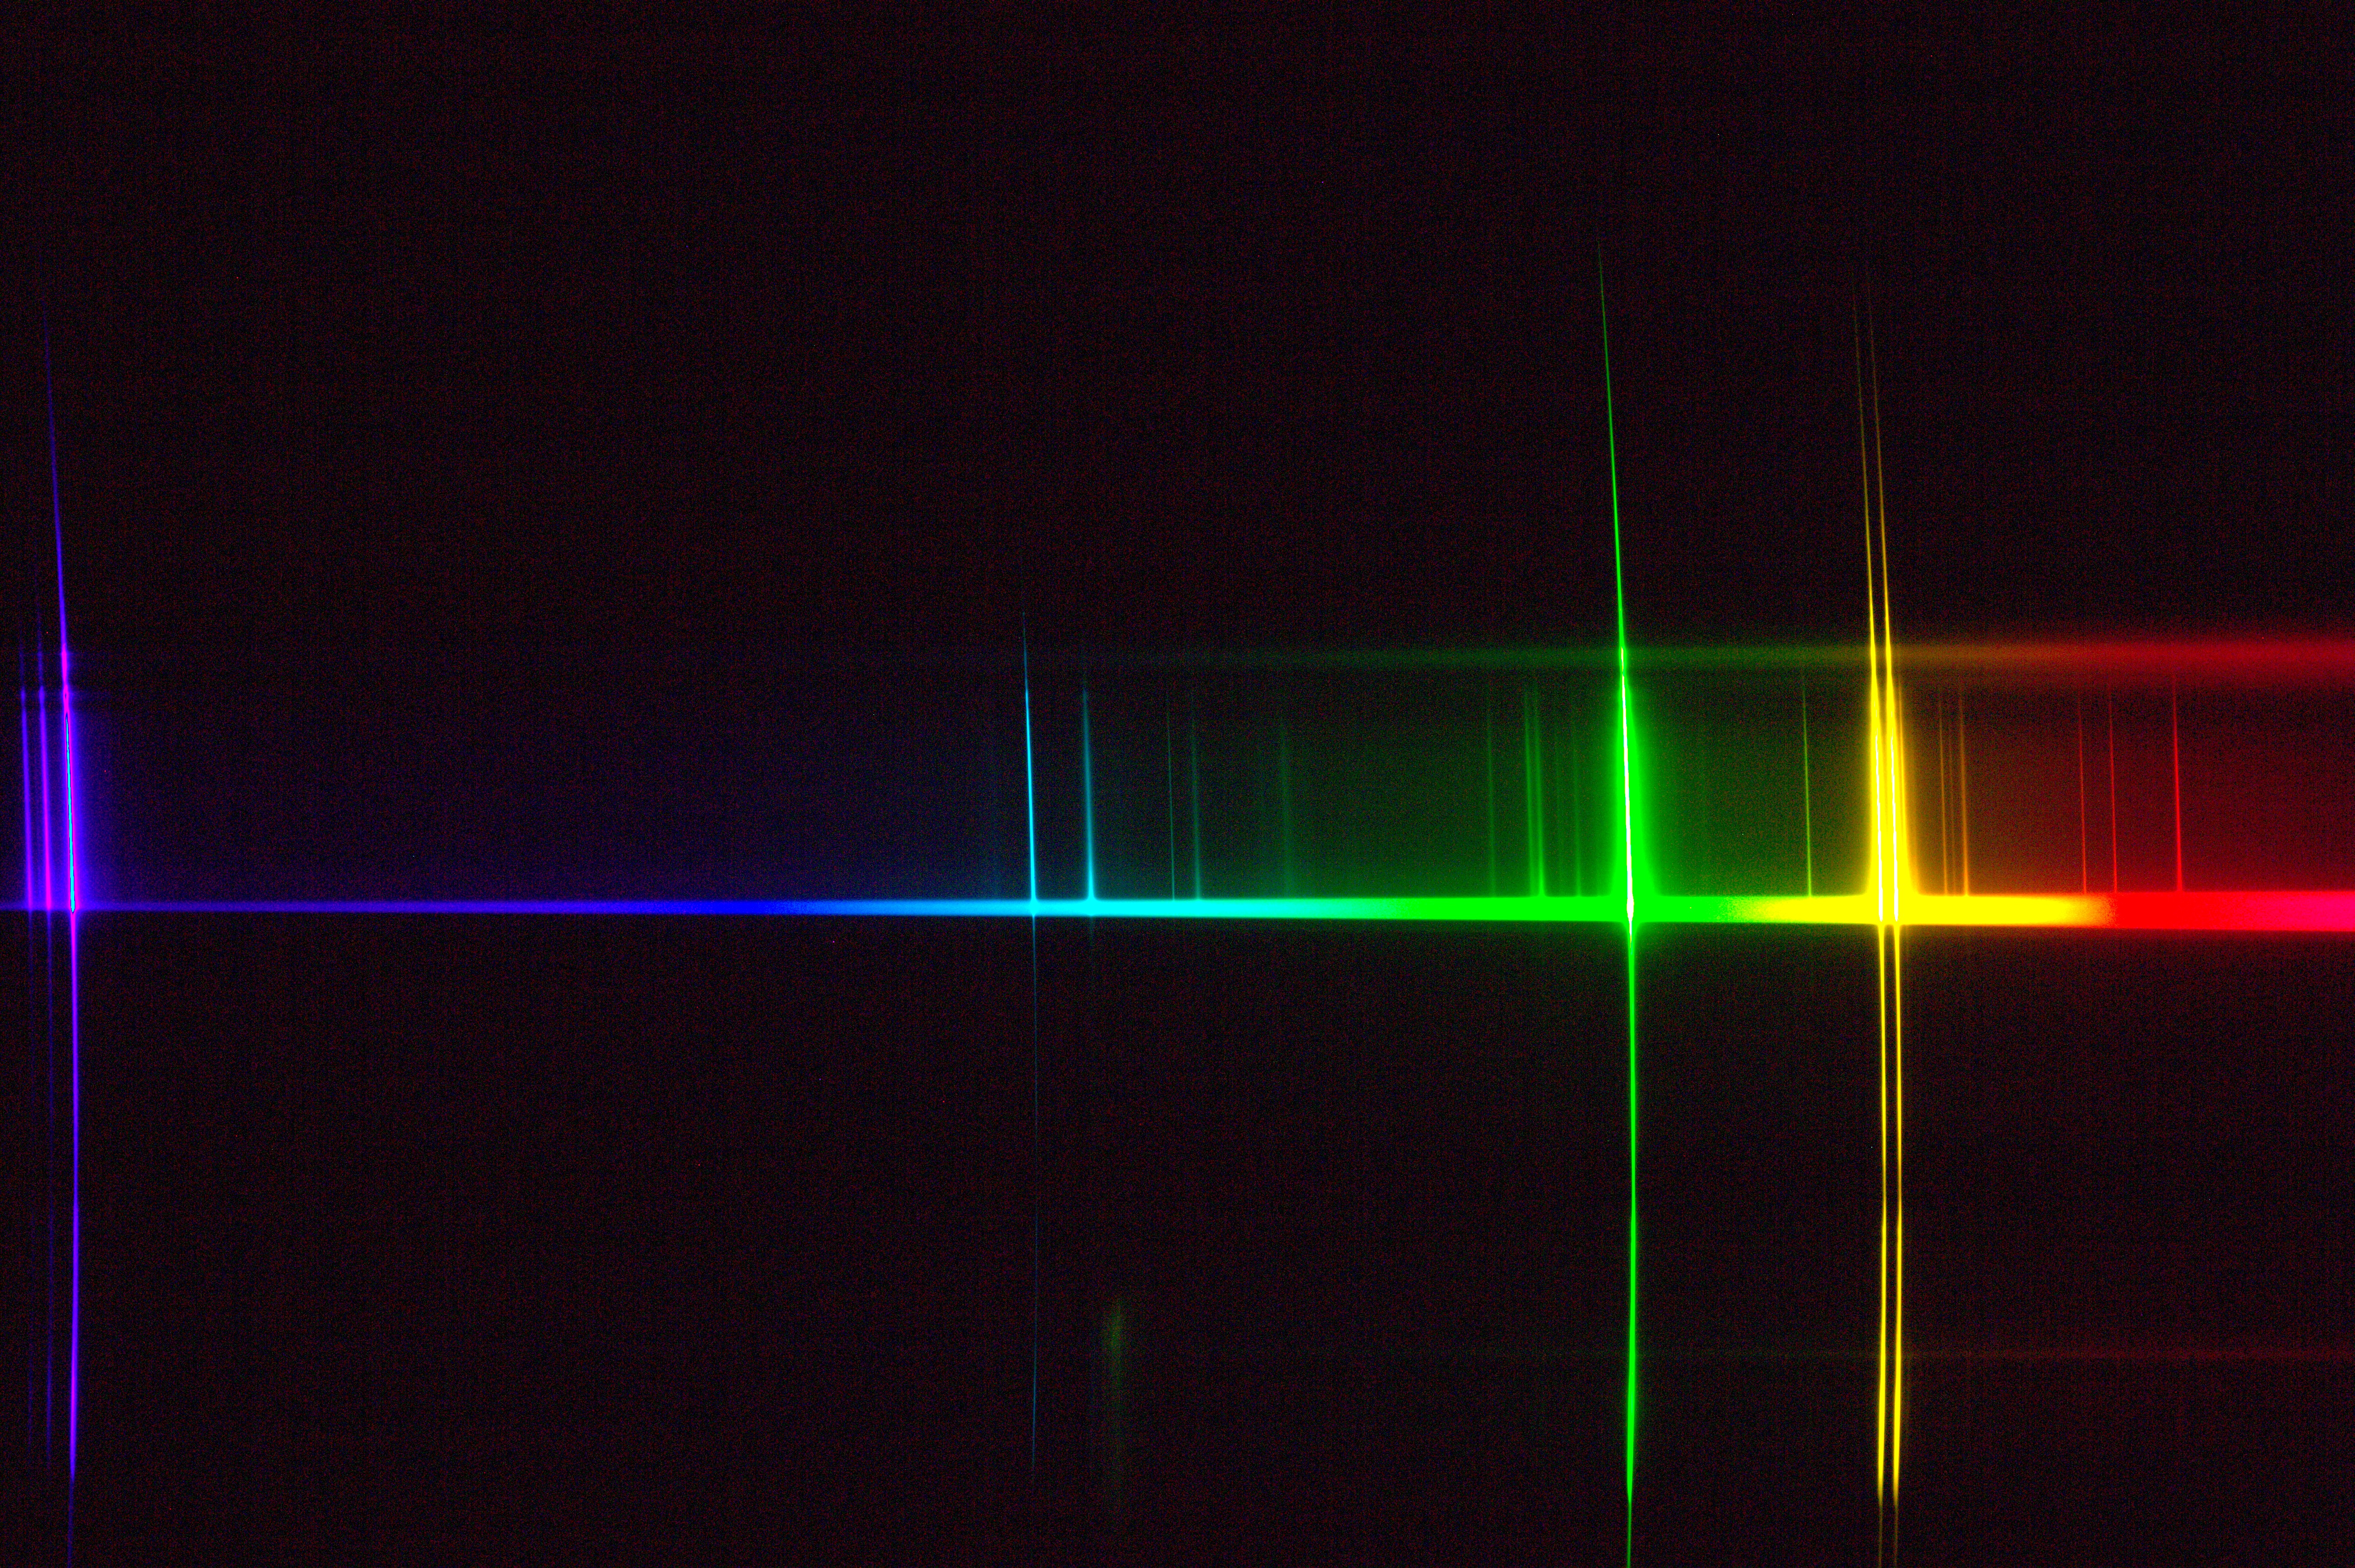
\includegraphics[width=0.9\linewidth]{data/323_50/323_50.jpg}
		\end{minipage}
		\caption{Фотографии спектров неоновой лампы (слева: выдержка 1 с; справа: выдержка $1/50$ с).}
		\label{fig:calibration_photo}
	\end{figure}
	
	\begin{minipage}{\textwidth}
		\begin{minipage}[]{0.6\textwidth}
			\centering
			\includegraphics[width=1.0\linewidth]{gen/calibration.pdf}
			\captionof{figure}{Зависимость длины волны от номера пикселя на фотографии.}
		\end{minipage}
		\hfill
		\begin{minipage}[]{0.39\textwidth}
			\centering
			\footnotesize
			\input{gen/calibration.tex}
			\captionof{table}{Данные калибровки спектра.}
		\end{minipage}
	\end{minipage}
	
	\begin{figure}[H]
		\centering
		\includegraphics[width=0.8\linewidth]{data/323_1s/spectrum.png}
		\caption{Откалиброванный график спектра неоновой лампы.}
		\label{fig:calibration_spectrum}
	\end{figure}
	
	Для известных линий неона составляется таблица, по которой производится интерполяция длины волны от номера пикселя.
	
	\subsection*{Измерение линий поглощения}
	
	\begin{figure}[H]
		\centering
		\includegraphics[width=0.8\linewidth]{data/326_2/merged.png}
		\caption{Фотографии спектров лампы (сверху: без кюветы с йодом; снизу: с кюветой с йодом).}
		\label{fig:iodine_photo}
	\end{figure}
	
	\begin{figure}[H]
		\centering
		\includegraphics[width=0.8\linewidth]{data/326_2/spectrum.edit.png}
		\caption{Откалиброванный график спектра поглощения паров йода.}
		\label{fig:iodine_spectrum}
	\end{figure}
	
	В спектре наблюдается множество пиков поглощения. Выделим отсюда серии Деландра. 
	
	\begin{table}[H]
		\footnotesize
		\input{gen/series.tex}
		\caption{Серии Деландра.}
		\label{tab:data}
	\end{table}
	
	\begin{figure}[H]
		\centering
		\includegraphics[width=0.8\linewidth]{gen/series.pdf}
		\caption{Положения пиков поглощения от номера $n_2$.}
		\label{fig:series}
	\end{figure}
	
	При росте $n_2$ наблюдается усиление ангармонизма, из-за чего энергетическое расстояние между линиями уменьшается.
	
	\begin{table}[H]
		\footnotesize
		\input{gen/mnk.tex}
		\caption{Параметры аппроксимации серий Деландра.}
		\label{tab:mnk}
	\end{table}
	
	Аппроксимируя начала серий прямыми $\nu = a n_2 + b$ получим:
	$a = (2.8 \pm 0.2)$ ГГц.
	Тогда $h \nu_2 = h a = (12.0 \pm 0.7)$ мэВ.
	
	Оценить значения $h \nu_1$ (энергии колебательного кванта основного состояния \figref{fig:delandr_series}) можно по разностям энергий между одинаковыми $n_2$ разных серий. Однако, эта разность сильно зависит от точности определения пика поглощения, соответствующего $n_2 = 0$ для обоих серий.
	Вычисляя для двух разностей получаем: $[ 27 ; 66 ]$ мэВ.
	
	Также можно оценить значение энергии электронного перехода. Перепишем \eqref{eq:lines} для коэффициентов аппроксимации:
	$$ h b_0 = (E_2 - E_1) + \frac{1}{2} (h \nu_2 - h \nu_1) \quad \Rightarrow \quad \Delta E = h b_0 - \frac{1}{2} (h \nu_2 - h \nu_1) = (2.17 \pm 0.02) \text{ эВ} $$
	Отметим, что большая погрешность $h \nu_1$ компенсируется малым вкладом в величину $\Delta E$.
	
	Оценка \eqref{eq:relation} для йода дает соотношение $\frac{h \nu_2}{\Delta E} = 1.5 \cdot 10^{-3}$. Из наших результатов $\frac{h \nu_2}{\Delta E} = 5.5 \cdot 10^{-3}$.
	\section*{Заключение и выводы}
	
	Работа подтверждает дискретность спектра поглощения молекулярного йода. Получены первые три серии Деландра.
	
	Получено значение кванта энергии колебаний первого возбужденного состояния молекулы:
	$$h \nu_2 = h a = (12.0 \pm 0.7) \text{ мэВ}.$$
	Получена оценка по порядку величины для кванта энергии колебаний основного состояния молекулы:
	$$h \nu_1 = (10 \div 100) \text{ мэВ}. $$
	Также оценено значение энергии электронного перехода
	$$E_2 - E_1 = (2.17 \pm 0.02) \text{ эВ}. $$

	
\end{document}
